\documentclass{article}
\usepackage[table,x11names,dvipsnames,table]{xcolor}
\usepackage{comment}
\usepackage{graphicx}
\graphicspath{ {./Images/} }

\usepackage{float}
\usepackage{hyperref}

\title{Het medisch vaststellen van de ABCDE lijst met een Arduino Due \thanks{Opdracht van de Hogeschool Utrecht voor het project R2D2 2019-2020}}
\author{Oscar Kromhout en Vincent van Setten\\ Team 3}

\date{April, 2020}


\begin{document}

\begin{titlepage}
	\centering
	\maketitle
	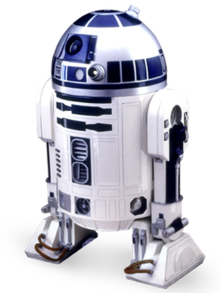
\includegraphics[scale=2.0]{title.png}
	\clearpage
\end{titlepage}

\tableofcontents
\clearpage 
\section{Samenvatting}
Hierin worden het onderzoek samengevat. Hier moeten sowieso de conclusies en resultaten in voor komen. De samenvatting moet onafhankelijk te lezen zijn en is bedoeld om een globaal overzicht te bieden.
	
\section{Inleiding}
De hoofdvraag van ons onderzoek gaat over het afwerken van de medische A.B.C.D.E. lijst. Met deze lijst bepalen medici in wat voor medische noodsituatie iemand verkeerd, en kan worden bepaald hoeveel hulp iemand nodig heeft. Een aantal van deze onderdelen kunnen worden gecontroleerd met sensoren. Denk hierbij aan temperatuur, hartslag of zuurstofsaturatie. Maar bij een groot deel is dit erg lastig met sensoren op te lossen en is het verstandig daar een menselijk oog aan te pas te laten komen. Het is dus handig als medisch personeel op afstand zou kunnen meekijken via een robot om iemands medische staat te controleren. Hiervoor willen wij deelonderzoek gaan uitvoeren naar de mogelijkheid een Arduino Due te gebruiken in combinatie met een camera. Om de scope van ons onderzoek te verkleinen doen we geen onderzoek naar het versturen van deze beelddata, maar wel naar het bufferen van deze beelddata zodat het in de toekomst verstuurd zou kunnen worden. 
Uit deze context hebben wij de volgende hoofdvraag afgeleid: 
Welke camera, compatibel met de Arduino due en onder de 28 euro, is het meest geschikt om de toestand van een patiënt te fotograferen of filmen en dit zo vlot en accuraat mogelijk lokaal te bufferen op het RAM geheugen van de Arduino due om wanneer het gebufferd kan worden, door te kunnen sturen naar medisch personeel voor de medische vaststelling van de A en D van de ABCDE lijst? 
Om deze hoofdvraag te beantwoorden hebben wij het onderverdeeld in 8 deelvragen. Deze lopen we systematisch en volgordelijk af om op die manier tot een antwoord op de hoofdvraag te komen. De deelvragen luiden als volgt:
\begin{enumerate}
	\item Bestaan er camera’s op de markt die geschikt zijn voor de Arduino Due, maar onder de 28 euro zijn?
	\item Welke factoren beïnvloeden welke camera het meest geschikt is voor onze toepassing? 
	\item Als er camera’s bestaan die aan onze geschiktheidseisen voldoen, welke zou dan het meest geschikt zijn voor deze toepassing? 
	\item Heeft de Arduino Due genoeg intern geheugen om één frame te bufferen met de meest geschikte camera? 
	\item Wat is het maximale aantal frames dat wij met de gekozen camera kunnen bufferen op het RAM geheugen van de Arduino Due? 
	\item Kan alles van de A {\&} D van de ABCDE lijst gecontroleerd worden met een foto of filmpje? 
	\item Wat moet medisch personeel zien op een filmpje of foto om erachter te komen wat er medisch nodig is voor de A {\&} D van de ABCDE lijst? 
	\item Hoeveel frames moeten we bufferen om het voor medici mogelijk te maken, zover het mogelijk is via beelden, de A {\&} D controle te doen? 
\end{enumerate}
De precieze uitwerking van deze deelvragen wordt beschreven in het hoofdstuk “Opzet en Uitvoering van het onderzoek”.
De doelgroep van ons onderzoek zijn tweedejaars technisch informatica studenten. Dit onderzoek moet immers weer opnieuw worden gebruikt in de hierop volgende jaren tijdens het R2D2 project.


\section{Literatuurverkenning}
We hebben een tweetal aan relevante research documenten gevonden.
De eerste hiervan is “Surveillance Robot Using Arduino Microcontroller, Android APIs and the Internet”. In dit onderzoek wilden ze een live video feed gebruiken voor een surveillance robot. In dit document gebruikten ze een android telefoon om de video feed te realiseren(het was gewoon een telefoon verbonden met een robot). 
Het tweede onderzoek is genaamd “Spy Robot Wireless Video Surveillance using Arduino”. 
In dit onderzoek willen ze ook een live feed opstellen. In dit onderzoek was het doel om een robot te maken die op afstand kon surveilleren, zodat hier geen mensen op het spel worden gezet in, bijvoorbeeld, een oorlog op het terrein van de vijand. 
In dit onderzoek hebben ze deze video feed gerealiseerd met een IP-camera, die zelf de beelden verstuurd via wifi. 

\section{Probleemstelling}
Filmen met een camera, deze data verwerken en deze data opslaan zijn zware taken voor een computer. We hebben een camera nodig die het mogelijk maakt op een Arduino te kunnen filmen. Deze beelden moeten van voldoende kwaliteit en kwantiteit voor medisch personeel zijn. Als we eenmaal in staat zijn om met een camera geschikte beelden te maken met een Arduino Due, moeten we die beelden ook nog kunnen bufferen om eventueel door te zenden naar een derde partij. We doen dus ook onderzoek naar het opslaan van deze hoeveelheid data op de geringe dataopslag van een Arduino Due. Verder moeten we weten wat dan een geschikte foto c.q filmpje is voor medisch personeel. Anders weten we niet hoeveel frames we precies moeten bufferen. Wij willen te weten komen welke camera onder de 28 euro het meest aan onze eisen voldoet, zodat wij dit mogelijk kunnen maken. 

\begin{comment}
Deze tabel kan volgensmij wat schoner. Kan iemand er even naar kijken. Niels misschien?
\end{comment}

\begin{table}[H]
	\centering
	\section{Begrippenlijst}
	\rowcolors{2}{gray!10}{white}
	\begin{tabular}{ |p{2cm}|p{10cm}| } 
			
		\hline 
		\textbf{Begrip} 		& \textbf{Definitie/Verklaring} \\
		\hline
		\hline

		Arduino Due 			& Een microcontroller board voor de cortex-m3 processor. \\ 
		
		\hline

		ABCDE lijst 			& De ABCDE lijst is een lijst die medisch personeel afgaat om zo de meest urgente problemen eerst af te handelen en niks over het hoofd te zien. \\
		
		\hline
		
		De A van de ABCDE lijst & De ‘A’ staat voor airway. Hier controleert medisch personeel of de luchtwegen vrij zijn. \\
		
		\hline
		
		De D van de ABCDE lijst & De ‘D’ staat voor disability. Hier controleert medisch personeel of de persoon bij bewustzijn is en of de persoon nog kan reageren op impulsen. \\
		
		\hline
	 
		\end{tabular}
		\caption{Begrippenlijst}
		\label{table:1}
	\end{table}

\section{Theorie en hypothese}
Voor ons onderzoek als totaal hebben wij geen hypothese. Voor deelvraag 4 echter wel. Om deze deelvraag te beantwoorden gaan we gebruik maken van een toetsend onderzoek. We stellen de hypothese dat de Arduino Due voldoende RAM geheugen heeft om 1 frame op te slaan. Deze frames moeten immers bewaard worden om eventueel later te versturen naar een medisch operator. Dit versturen valt buiten de scope van ons onderzoek.
We ontwerpen onze software alsof de Arduino Due voldoende geheugen heeft om de frame van de gekozen camera op te slaan en testen vervolgens of dit lukt. Vervolgens maken we 20 foto’s, als de Arduino dan niet vastloopt of data verliest en steeds de vorige foto netjes overschrijft weten we dat we de code kunnen gebruiken om camerabeeld te bufferen op een Arduino Due. 

De hypothese is dus als volgt: \textit{"De arduino Due heeft voldoende Ram geheugen om 1 frame op te slaan die gemaakt is met de gekozen camera."}

\section{Opzet en uitvoering van het onderzoek}
De opzet van dit deel onderzoek verloopt volgens de waterval methode. We lopen stapsgewijs door de deelvragen heen en beantwoorden de vragen door middel van bijbehorende onderzoeksmethoden. Uiteindelijk is er dan een conclusie die we kunnen verbinden aan de hoofdvraag om deze te beantwoorden.

Omwille van de leesbaarheid hebben we de deelvragen met hun bijbehorende toetsmethode hieronder in kopjes samengevat. 
\begin{enumerate}
	\item Bij de eerste deelvraag doen we een exploratief onderzoek. We gaan op het internet zoeken naar camera’s en kiezen 5 camera’s die veel voorkomen om nader te onderzoeken. Als Covid-19 niet had plaatsgevonden waren we ook naar een aantal winkels en school gegaan om experts op het gebied hiernaar te vragen (Wouter van Ooijen bv.). Maar dat werd nu wat lastig dus beperken we ons tot veel voorkomende camera’s op het internet. Via deze \href{https://www.open-electronics.org/a-complete-guide-to-arduino-based-video-camera/}{website} hebben we een hoop goede camera’s kunnen vinden.
	\item Vraag 2 beantwoorden we door met elkaar te sparren en te beredeneren welke factoren voor het bufferen en gebruik op microcontrollers belangrijk zijn voor een camera.
	\item Vraag 3 beantwoorden we door bij iedere gekozen factor een eis te stellen waar de camera aan moet voldoen. Dan gaan we beredeneren welke camera we het beste kunnen kiezen voor ons onderzoek.
	\item Vraag 4 gaan we beantwoorden volgens het toetsend onderzoek zoals beschreven in het hoofdstuk “theorie en hypothese.” We nemen aan dat er voldoende geheugen is op Arduino om 1 frame op te slaan, schrijven hier onze code voor, en gaan toetsen of dat dit ook het geval is. Het toetsen bestaat uit 20 keer een foto maken, bekijken of de vorige foto wordt overschreven in het geheugen en bekijken of de Arduino niet vastloopt of data verliest.
	\item Vraag 5 kunnen we beantwoorden door middel van een observatie onderzoek. We weten inmiddels hoe veel ruimte 1 frame in neemt, en we weten hoeveel Ram geheugen we hebben op de Arduino Due. Vervolgens kunnen we uitrekenen hoeveel frames we moeten kunnen bufferen op de Arduino.
	\item Vraag 6 {\&} 7 gaan we beantwoorden door het aan een medisch expert te vragen. Medisch personeel kan precies vertellen wat men zou willen zien op een foto om de A {\&} D te kunnen beoordelen van de ABCDE lijst.
	\item Vraag 8 kunnen we beantwoorden nadat we het antwoord hebben op vraag 5 {\&} 6. Dit is dus een observatie onderzoek.  

\end{enumerate} 

\subsection{Conclusies Deelvragen}
In dit onderdeel bespreken we de conclusies waartoe we gekomen zijn uit ons deelonderzoek.

\subsubsection{Deelvraag 1 {\&} 2}
We hebben een aantal camera's gevonden en hebben de belangrijkste factoren die het antwoord op onze deelvragen beantwoorden.
Zie figure \ref{fig:deelvragen1en2}.
s

\begin{figure}[h]
	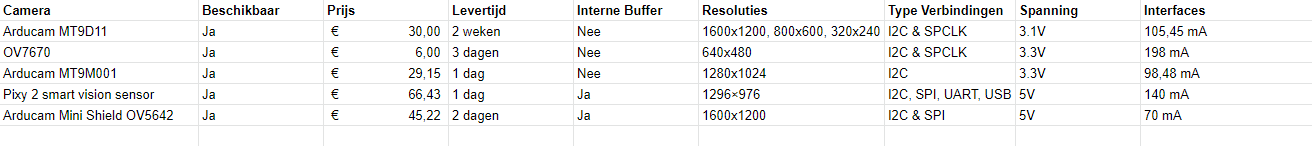
\includegraphics[width=40em]{table2}
	\centering
	\caption{Deelvragen 1 {\&} 2}
	\label{fig:deelvragen1en2}
	\end{figure}

In figure \ref{fig:deelvragen1en2} zie je een tabel met in de linkerkolom de 5 gekozen camera's. In de overige kolommen zie je de eigenschappen en in welke mate de betreffende camera deze eigenschap bezit.

Wij interpreteren de volgende factoren als van belang voor ons onderzoek:
\begin{itemize}
	\item \textbf{Beschikbaar}, is de camera nog te koop of op een andere manier te vinden?
	\item \textbf{Prijs}, de prijs van de camera, dit is een belangrijke factor omdat we tijdens de corona crisis maar €28,- per persoon te besteden hebben aan electronica. Daar kunnen we nog wel iets overheen omdat niet alle teamgenoten dat bedrag uitgeven maar we kunnen niet heel ver uitschieten.
	\item \textbf{Levertijd}, de tijd dat het kost tussen bestellen en het in huis hebben. Deze factor is ook vrij belangrijk geworden door de corona crisis. We moeten de camera wel op tijd in huis hebben om het onderzoek af te kunnen ronden en eventueel iets te bouwen.
	\item \textbf{Interne Buffer}, heeft de camera een buffer intern of niet? Deze buffer kan voor ons voordelen opleveren tijdens het coderen. Door een buffer te hebben kan het makkelijker zijn om plaatjes vanaf de camera op de Arduino te zetten. Dan hoeft dit proces namelijk niet hard realtime te gebeuren. Maar kan het gebeuren op een moment dat het ons uitkomt.
	\item \textbf{Resolutie}, welke resolutie heeft de camera? De resolutie kunnen we gebruiken om het aantal pixels te berekenen dat 1 plaatje zou bevatten. Daarmee kunnen we dan uitrekenen of het te bufferen is op het RAM geheugen voor we code en testen gaan schrijven.
	\item \textbf{Spanning}, hoeveel volt heeft de camera nodig? De hoeveelheid benodigde spanning is belangrijk om te weten. Als de camera namelijk teveel spanning vereist, zou dat betekenen dat we met relais en een externe stroombron moeten gaan werken om hem te gebruiken. Dat is gezien de €28,- per persoon die we hebben vanuit de opdrachtgever niet handig.
	\item \textbf{Interface}, met welke interface kunnen we de camera verbinden? Het type interface belangrijk vanwege de verbindingsmogelijkheden. Als de camera gebruik maakt van een interface die niet te gebruiken is icm een Arduino kunnen we de camera helemaal niet gebruiken. Verder is het fijn als er een interface gebruikt wordt waar al code voor bestaat binnen het bedrijf. Hier hoeven we dan geen tijd aan te besteden bij het onderzoek.
\end{itemize}


\section{Resultaten}
De onderzoeksvragen, theorie en hypotheses worden hier kort samengevat. Hier volgen nog geen interpretatie wel getalsmatige conclusies.

\section{Conclusie en discussie}
Hier worden de resultaten in verband gebracht met de vraagstelling en worden de conclusies en verbanden gelegd.

\section{Evaluatie}
Hier wordt het onderzoek geëvalueerd op product- en procesniveau. Er wordt dus gekeken naar de sterke en zwakke punten van het onderzoek, de leerervaringen en eventuele zaken die verkeerd zijn gegaan en in de toekomst anders zouden moeten. Verder wordt een onderzoekslogboek bijgevoegd waarin de dagelijkse besluiten en gebeurtenissen in staan.

\section{Aanbevelingen}
Hier kunnen eventuele aanbevelingen worden gedaan op basis van de conclusies en resultaten.

\section{Suggesties voor verder onderzoek}
Mochten er tijdens het onderzoek nieuwe vragen naar voren zijn gekomen of nog onbeantwoorde vragen overgebleven zijn dan kunnen hier suggesties worden aangegeven. Deze kunnen dan eventueel in een nieuwe onderzoek meegenomen worden.

\section{Literatuur}
In de literatuurlijst geef je op alfabetische volgorde aan welke literatuur je tijdens je onderzoek hebt gebruikt. Het is dan ook aan te raden om tijdens je onderzoek goed bij te houden welke bronnen je hebt gebruikt en wat je precies uit die bronnen hebt gehaald.

\section{Bijlagen}
Stukken die niet in je onderzoeksrapport past kan je in de bijlagen plaatsen. Denk hierbij aan vragenlijsten, observatieschema’s, codeerschema’s, brieven aan respondenten, etc.


\end{document}